\chapter{Metodología}

En este capítulo se describe la fuente de información que se emplea
para el desarrollo, así como los procesos a seguir para generar el asistente
descrito en el capítulo 1, cuya implementación se divide en cuatro componentes
fundamentales: Extractor de información, modelador de lenguaje, API de
comunicación y aplicación web. El objetivo es generar un sistema cuyos
componentes modulares puedan ser diseñados, desarrollados, modificados o
escalados.

El desarrollo de el asistente requiere el uso de múltiples lenguajes de programación,
frameworks y librerías, siendo los princiales: Python (transformers, llama\_cpp)
para usar y reentrenar los modelos LLM, además de para programar la API de
comunicación (FastAPI), Javascript (NextJS, React) para desarrollar la aplicación
web.

En la figura \ref{fig:esquema_general} se muestran los cuatro módulos del
sistema donde: El extractor de información realiza un proceso previo en el que
se recopilan los documentos, se extrae su contenido, se transforma en
\textit{embeddings} y, finalmente, se almacena en una base de datos; El
modelador de lenguaje recibe la pregunta, busca en la base de datos los
fragmentos de información relevante y se los proporciona al LLM, para que
genere la respusta; La API de comunicación, funge como intermediario entre la
aplicación web y el modelador de lenguaje, controlando el envió y recepción de
las preguntas y respuestas; Por último, la aplicación web es el medio de
interacción de los usuarios con el sistema, al tener forma de un chat es
posible realizar preguntas en lenguaje natural a través de cajas de texto, botones
y mensajes intuitivos.

\begin{figure}[]
    \centering
    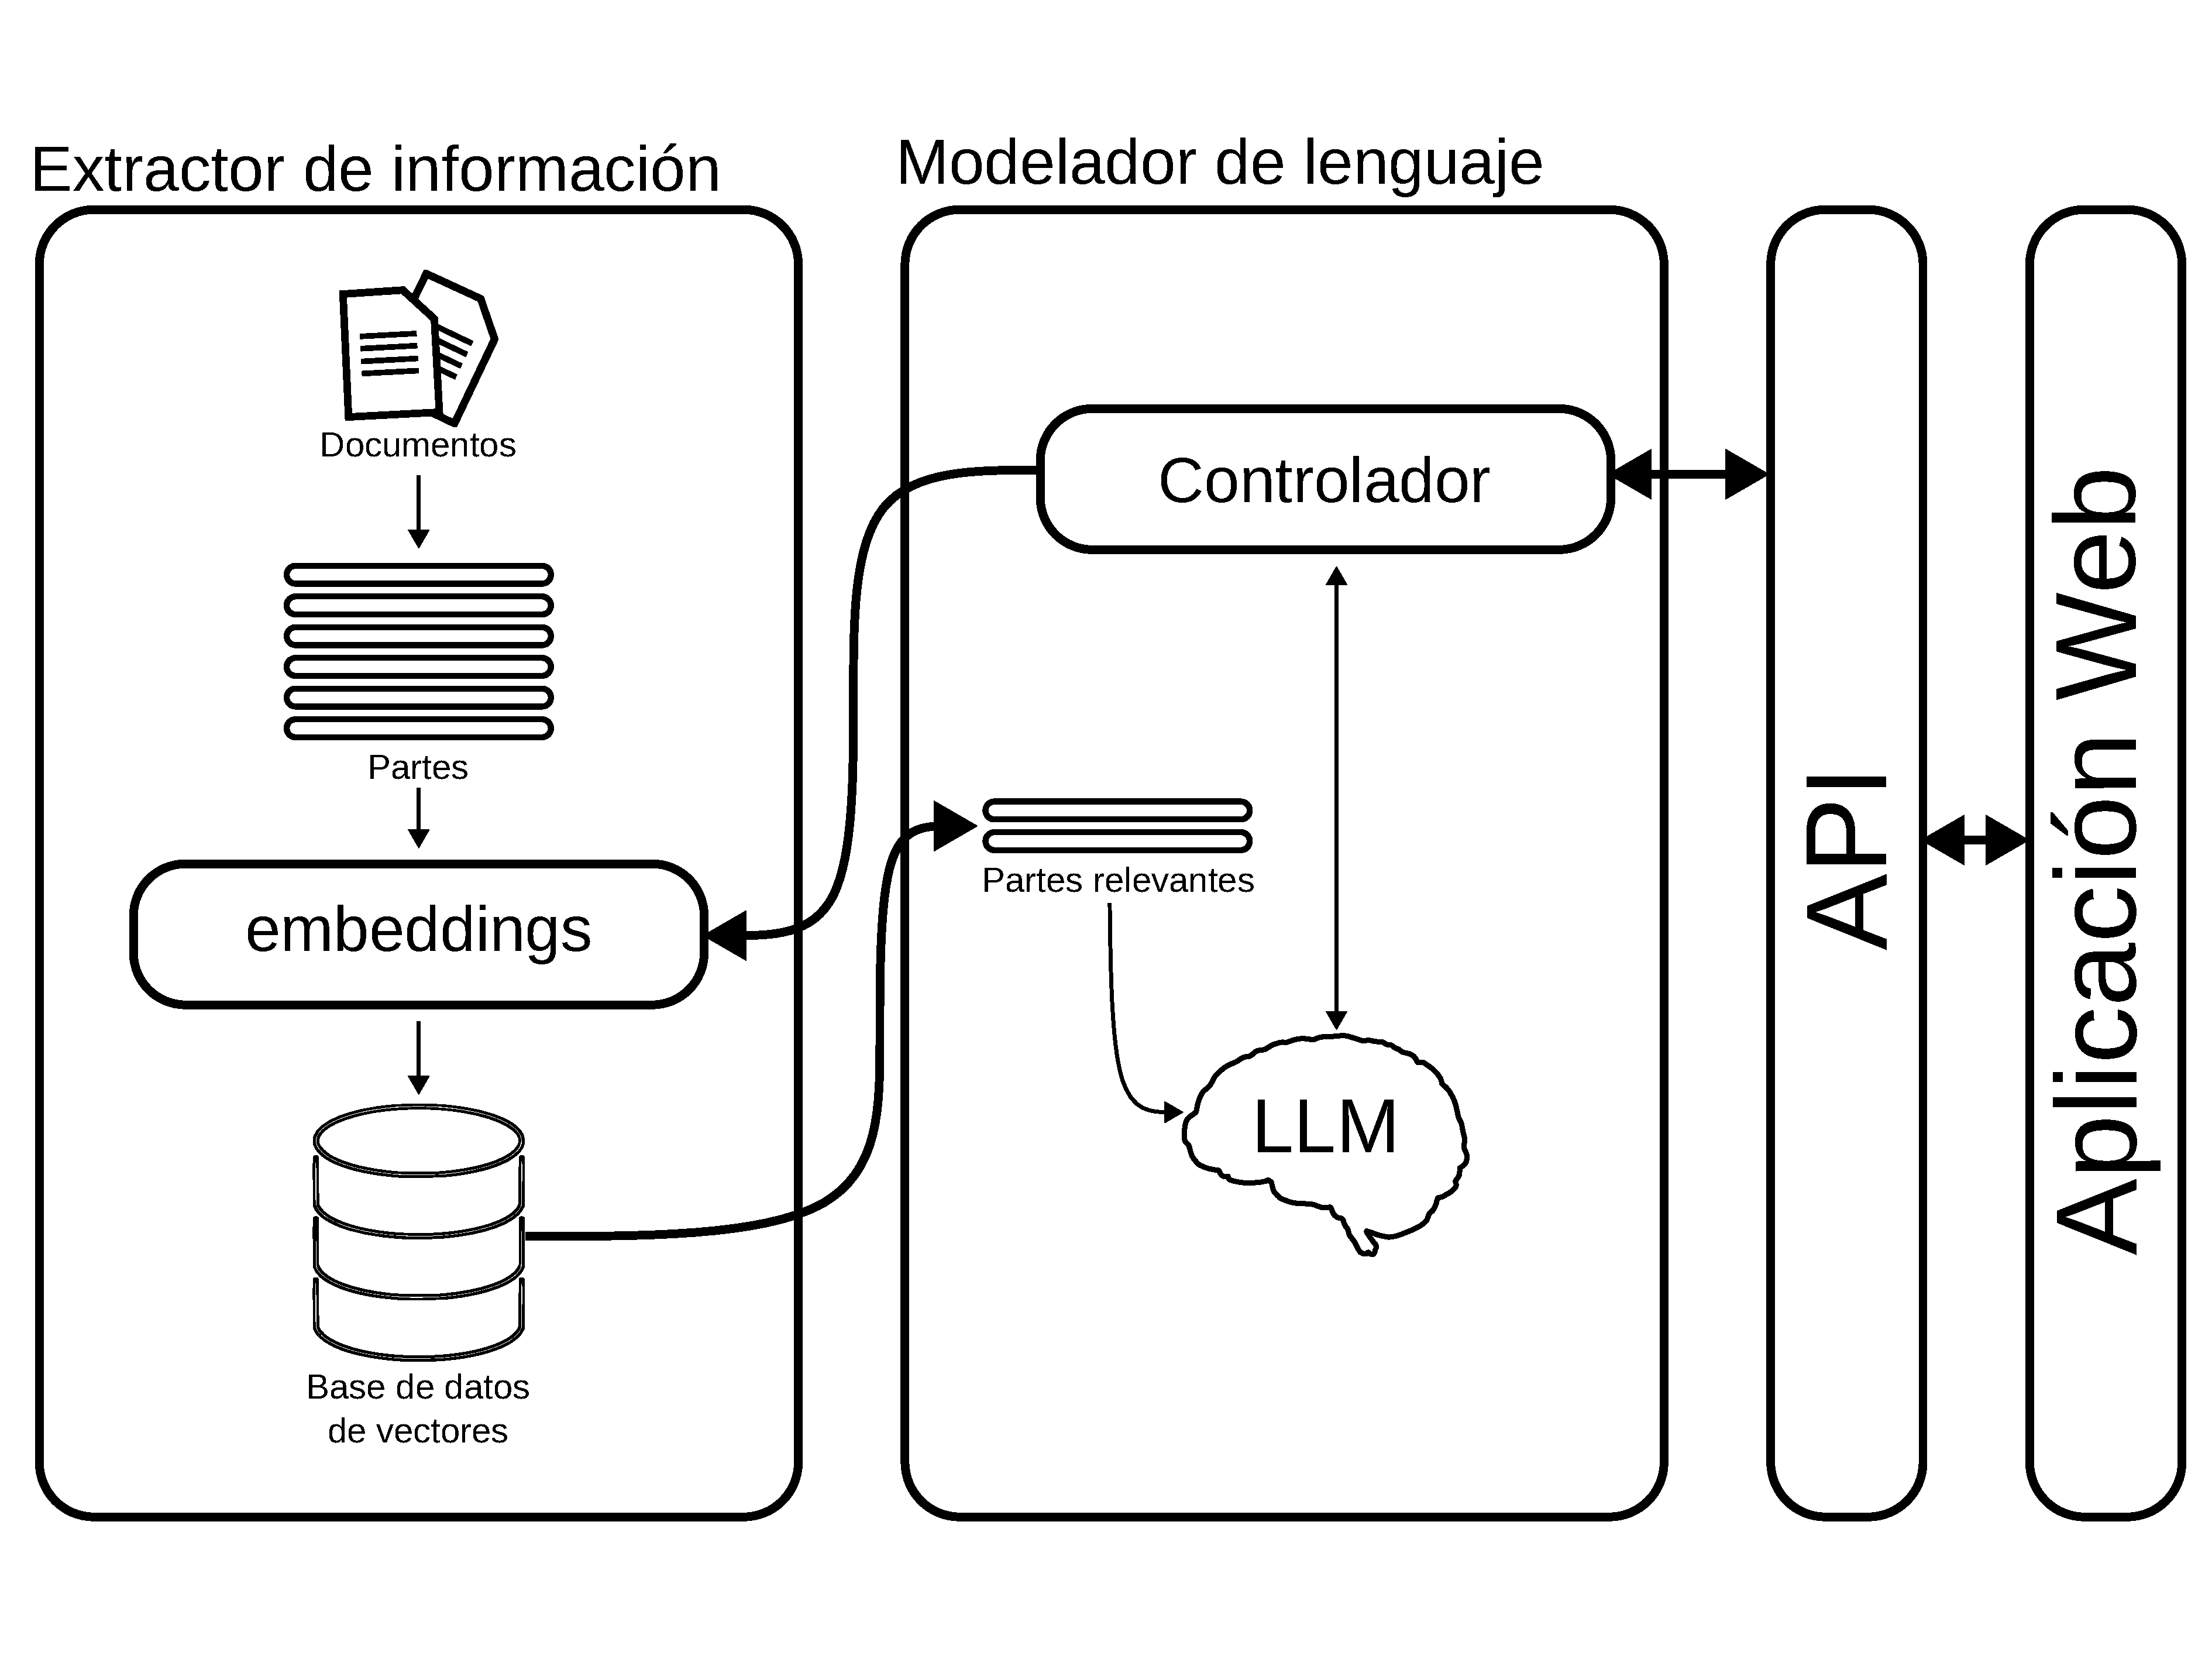
\includegraphics[width = 0.8\textwidth]{\DirFigCtres/esquema_general}
    \caption{Diagrama de componentes que conforman el sistema.}
    \label{fig:esquema_general}
\end{figure}

\section{Fuente de información}

El sistema está diseñado para responder preguntas de la normativa de la
Universidad de Guanajuato, esta normativa se encuentra disponible en la página
oficial de la universidad
\footnote{https://www.ugto.mx/gacetauniversitaria/normatividad/normatividad-vigente}
en forma de 22 documentos PDF individuales. Cada documento tiene un número
diferente de páginas, las cuales suman 511, representan 6.8MB de información y,
convertidas a texto, 168,011 palabras.

Los documentos son descargados manualmente y almacenados en un directorio,
para cada uno se utiliza el nombre del archivo como identificador.

**Incluir tabla con detalle de cada documento de la normativa**

\section{Extractor de información}

El funcionamiento del módulo de extracción de información comienzan con un
archivo en formato PDF y terminan con la creación de una base de datos de
embeddings de los fragmentos del documento. En la figura
\ref{fig:esquema_extractor} se observa la secuencia de procesamiento para un
archivo y la salida de cada una de las etapas.

\begin{figure}[]
    \centering
    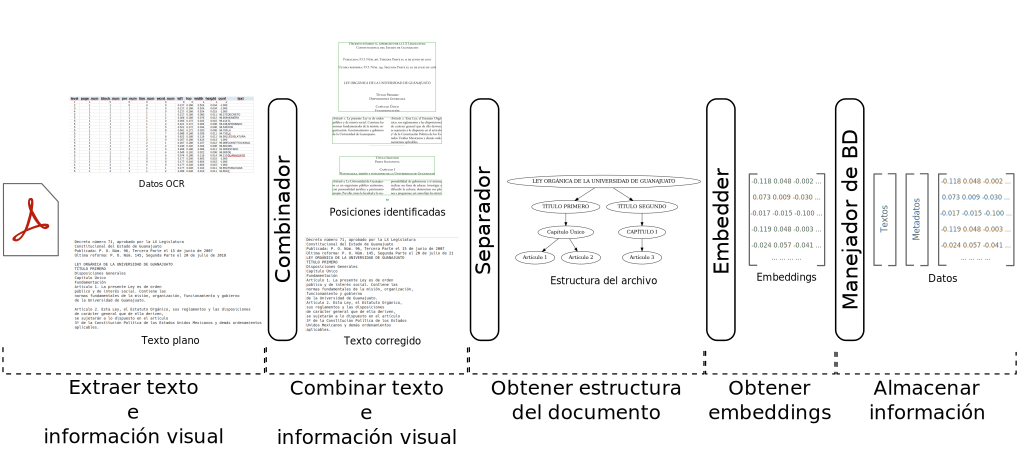
\includegraphics[width = 0.8\textwidth]{\DirFigCtres/esquema_extractor}
    \caption{Diagrama de extracción de información de un archivo PDF.}
    \label{fig:esquema_extractor}
\end{figure}

\subsection{Extraer texto e información visual}

El documento PDF debe convertirse a texto para su procesamiento, pero es
necesario conservar la información del formato y ubicación de los segmentos
para poder extraer la estructura del documento. Por lo anteior, se extraen dos
tipos de datos del archivo: texto plano e información visual relacionada con
el formato.

Para seleccionar las herramientas de extracción de texto plano se hizo un
análisis de aquellas que fueran de código abierto, considerando sus
deficiencias en la extracción de texto (ver Apéndice A). Se seleccionaron
PyPDF, porque es la herramienta más usada para esta tarea con Python, y
PdfPlumber, porque su extracción de texto es la más limpia y provee mecanismos
para extraer la información visual.

Primero se extrae el texto plano con PyPDF o PdfPlumber. En el caso de PyPDF
no se obtiene información visual que ayude a identificar los títulos, secciones
y encabezados, además en ocasiones modifica el orden del texto. Cuando se
emplea PdfPlumber, el texto va acompañado de la información visual del docuemto,
que consiste en la ubicación de cada palabra dentro del docuemnto.

Para obtener la información visual, cuando no se tiene, se utiliza la herramienta
Tesseract, la cual es un software de reconocimiento óptico de caracteres que
nos permite obtener la ubicación y texto de cada palabra dentro del documento.
Para emplear Tesseract, primero se convierte el documento a imágenes con
PDF2Image, las imágenes resultantes tienen una densidad de pixeles de 1000 DPIs.
Posteriormente, se usa la librería PyTesseract para obtiener información del
documento, específicamente, para cada palabra de la página obtiene: posición,
ancho, alto y texto predicho.

La librería PyTesseract ejecuta la herramienta Tesseract, desarrollada por
Google para hacer OCR. Esta herramienta puede reconstruir el texto del documento,
así como detectar las líneas, párrafos y secciones, sin embargo, con frecuencia
comete errores en la detección del texto y el ordenamiento. Para corregir
estos errores se opta por combinar el texto plano obtenido con PyPDF, con
la información de posición y tamaño devuelto por PyTesseract, de esta forma
obtenemos el texto correcto asociado a su ubicación y tamaño. Este proceso
se describe en el diagrama de la figura \ref{fig:texto_y_ocr}.

\begin{figure}[]
    \centering
    \includegraphics[width = 0.8\textwidth]{\DirFigCtres/esquema_texto_y_ocr}
    \caption{Detalle extracción de texto y características de OCR.}
    \label{fig:texto_y_ocr}
\end{figure}

Para el caso de PdfPlumber, la librería devuelve las mismas características que
PyTesseract, sin embargo, comete también errores en la agrupación y el
ordenamiento del texto, por ello se requiere realizar los pasos de "Crear
grupos para reconstruir el texto" y "Reconstruir texto" del diagrama de la figura
\ref{fig:texto_y_ocr}.

La tarea de agrupar el texto en secciones para reconstruirlo en el orden correcto
no es trivial, y es altamente dependiente del tipo de documento del
que se trata, es decir, el proceso descrito en el diagrama de las figuras
\ref{fig:reconstruccion_texto_1} y \ref{fig:reconstruccion_texto_2} funciona para
documentos con estructura similar, donde predomina el texto en una o dos
columnas con títulos centrados.

\begin{figure}[]
    \centering
    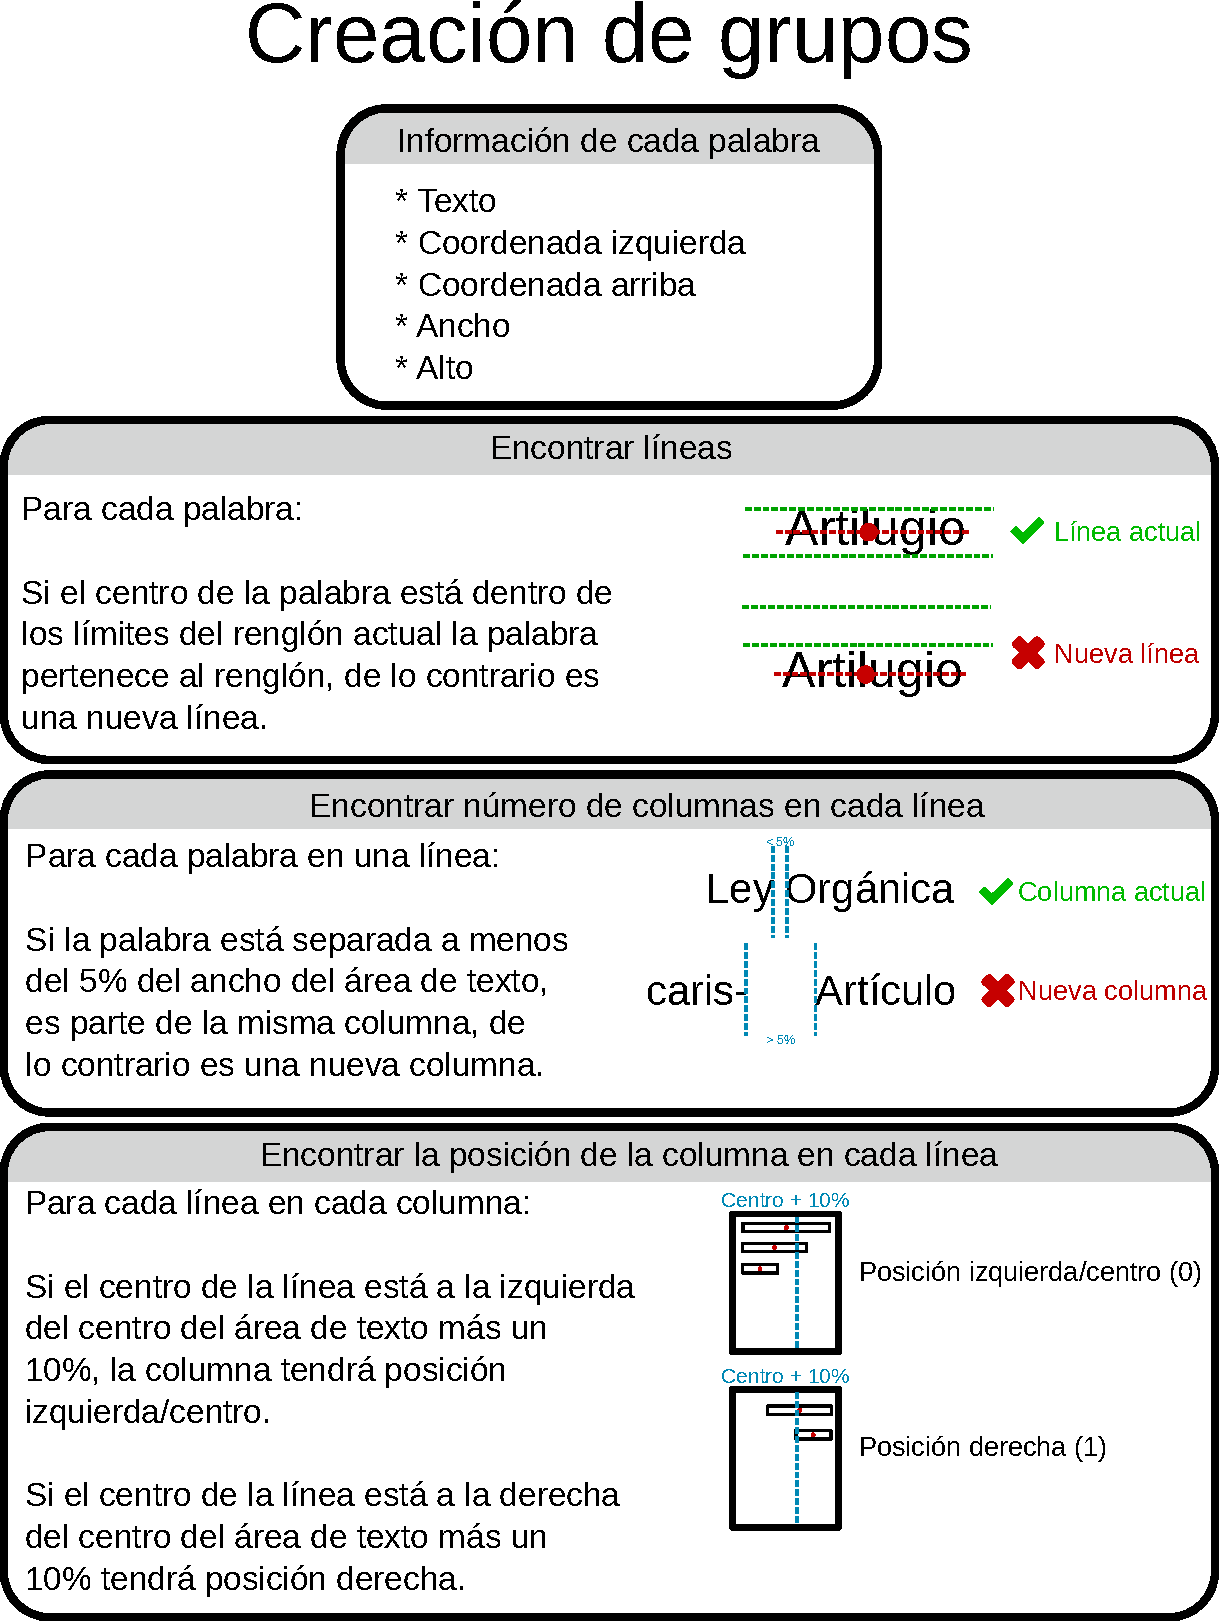
\includegraphics[width = 0.8\textwidth]{\DirFigCtres/reconstruccion_texto_ocr_1}
    \caption{Detalle de reconstrucción de texto del documento (Pt. 1).}
    \label{fig:reconstruccion_texto_1}
\end{figure}

\begin{figure}[]
    \centering
    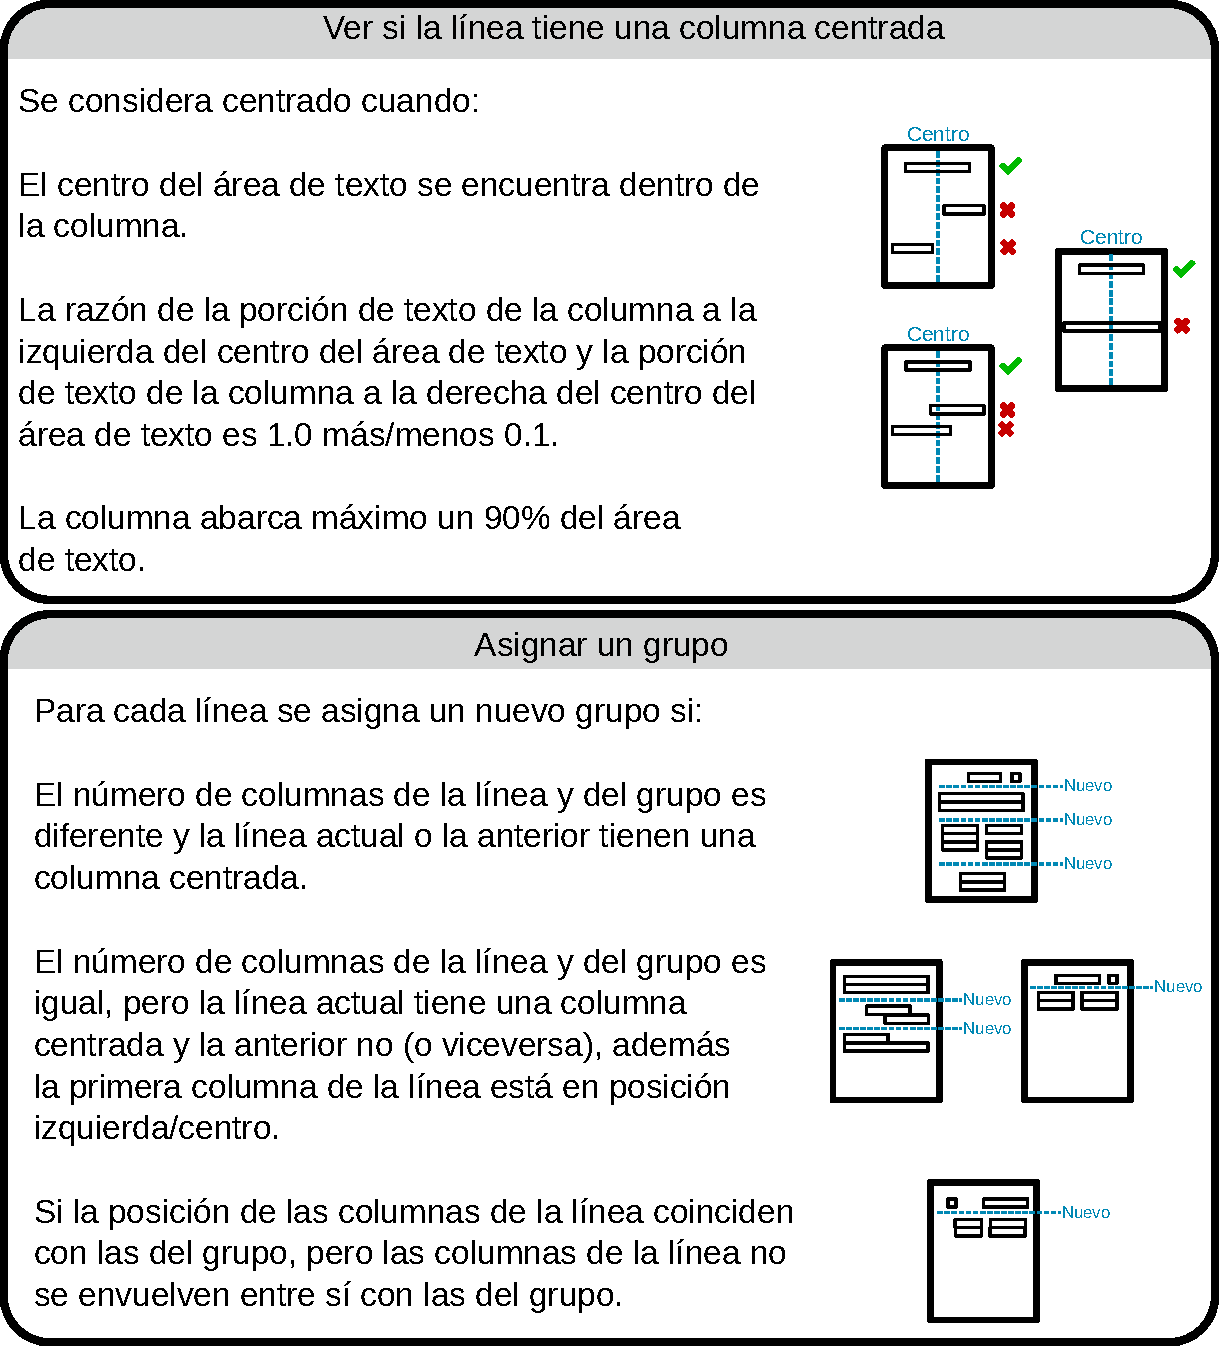
\includegraphics[width = 0.8\textwidth]{\DirFigCtres/reconstruccion_texto_ocr_2}
    \caption{Detalle de reconstrucción de texto del documento (Pt 2).}
    \label{fig:reconstruccion_texto_2}
\end{figure}

Una vez realizada la agrupación de los elementos de la página, es posible reconstruir
el texto respetando el orden normal de lectura. Este texto usualmente contiene
errores de detección que serán corregidos al combinar el texto reconstruido
con OCR con el texto plano extraido con PyPDF.

\subsection{Combinar texto e información visual}

Cuando se usa PdfPlumber, este proceso no es necesario, pues la librearía ya
devuelve el texto correcto asociado a su informació visual de posición y tamaño,
sin embargo, cuando se usa PyPDF y PyTesseract, es necesario combinar estas dos
fuentes de información para obtener el texto e información visual correctas,
el objetivo es tener la posición de cada palabra asociada con su texto correcto,
de esta forma se podrá distinguir entre diferentes elementos, como títulos,
párrafos, entre otros.

El proceso de combinación requiere las cadenas de texto extraídas por los dos métodos:
la cadena proporcionada por PyPDF y la cadena reconstruida con la información
visual, como se muestra en la figura \ref{fig:reconstruccion_texto_2}. Ambas cadenas se
separan por palabra y se pasan a la librería Difflib, la cual aplica el algoritmo
Ratcliff-Obershelp, también conocido como Coincidencia de patrones Gestalt, para
comparar dos cadenas y encontrar sus diferencias.

Si se analizan los patrones de salida de la librería Difflib, es posible
corregir las palabas detectadas con OCR utilizando las palabras extraidas directamente
del texto, los detalles de esta implementación se explican en las figuras
\ref{fig:esquema_combinacion_txt_ocr_1} y \ref{fig:esquema_combinacion_txt_ocr_2}.
En escencia, se considera la palabra obtenida con PyPDF como la correcta,
se compara contra la palabra obtenida con OCR y si es diferente se sobreescribe.

\begin{figure}[]
    \centering
    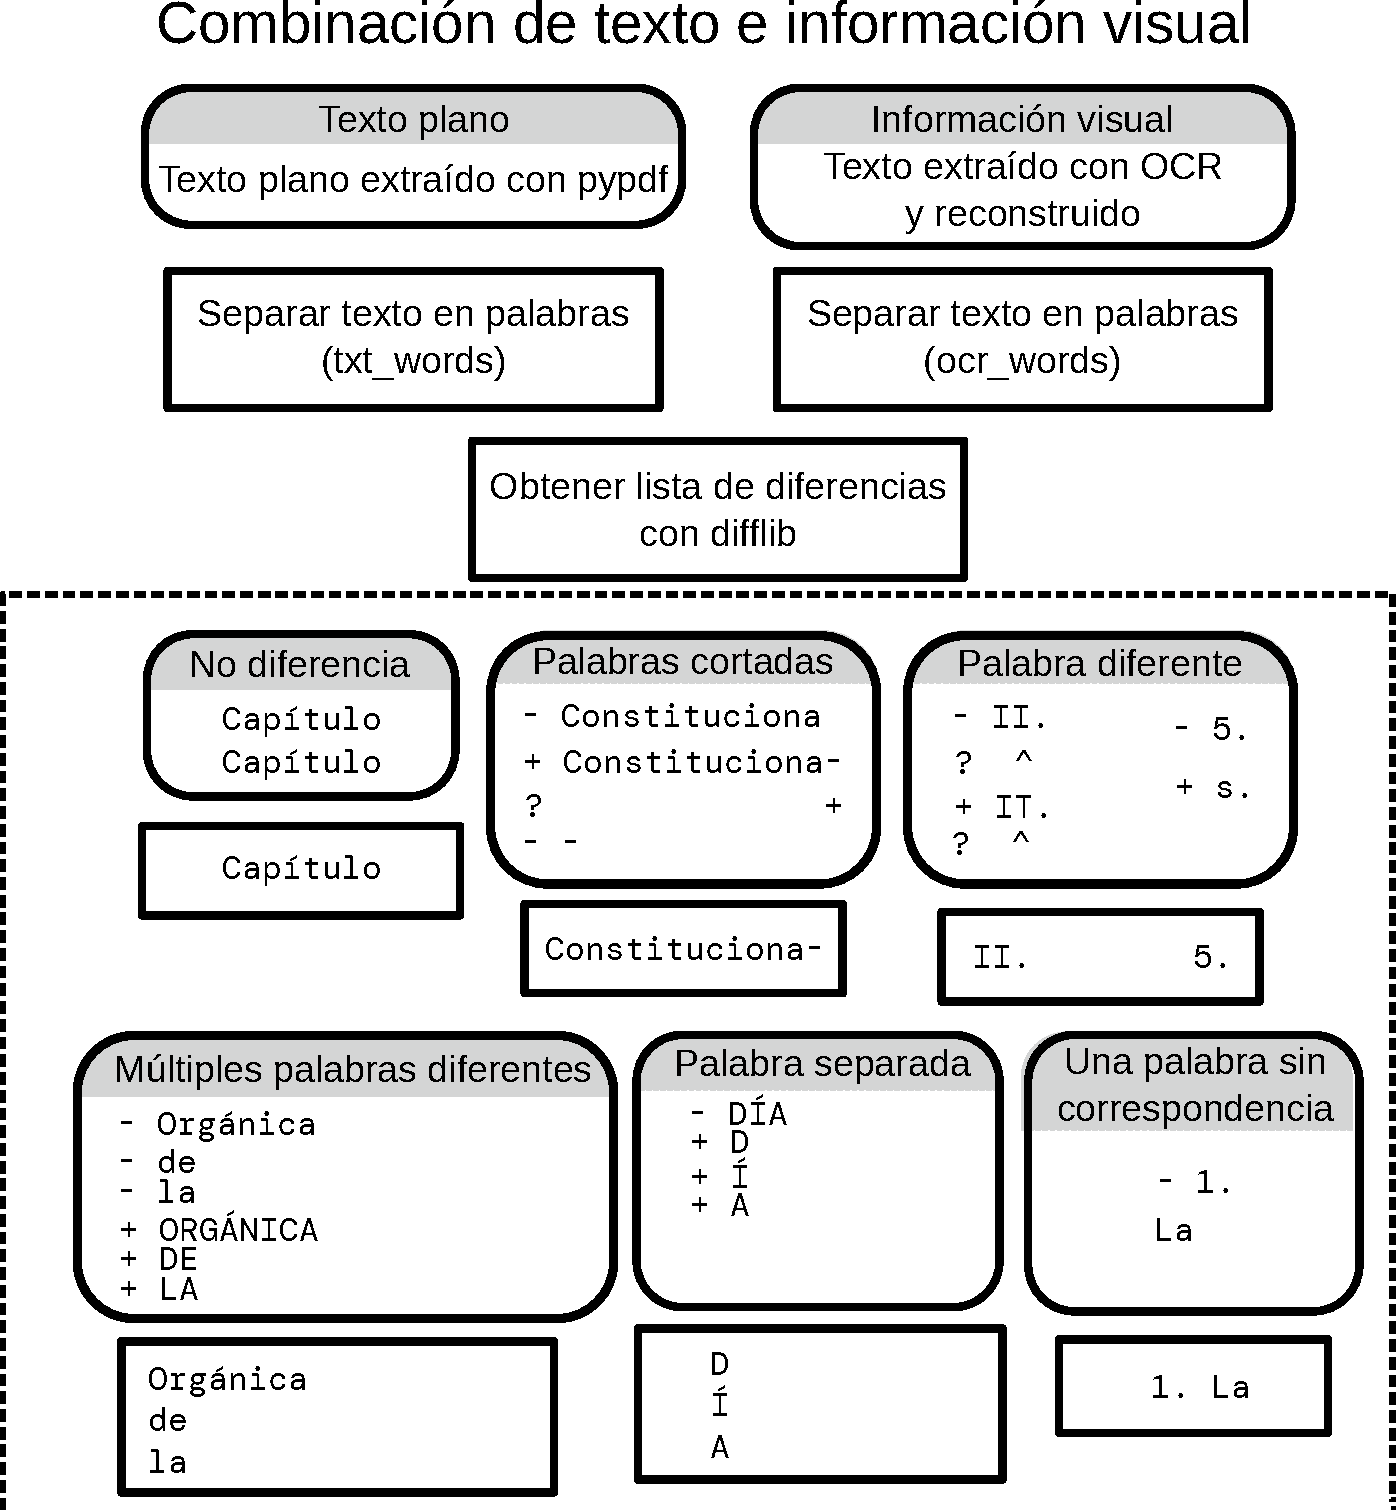
\includegraphics[width = 0.8\textwidth]{\DirFigCtres/combinacion_texto_ocr_1}
    \caption{Detalle de combinación de teto plano con información de OCR (Pt 1).}
    \label{fig:esquema_combinacion_txt_ocr_1}
\end{figure}

\begin{figure}[]
    \centering
    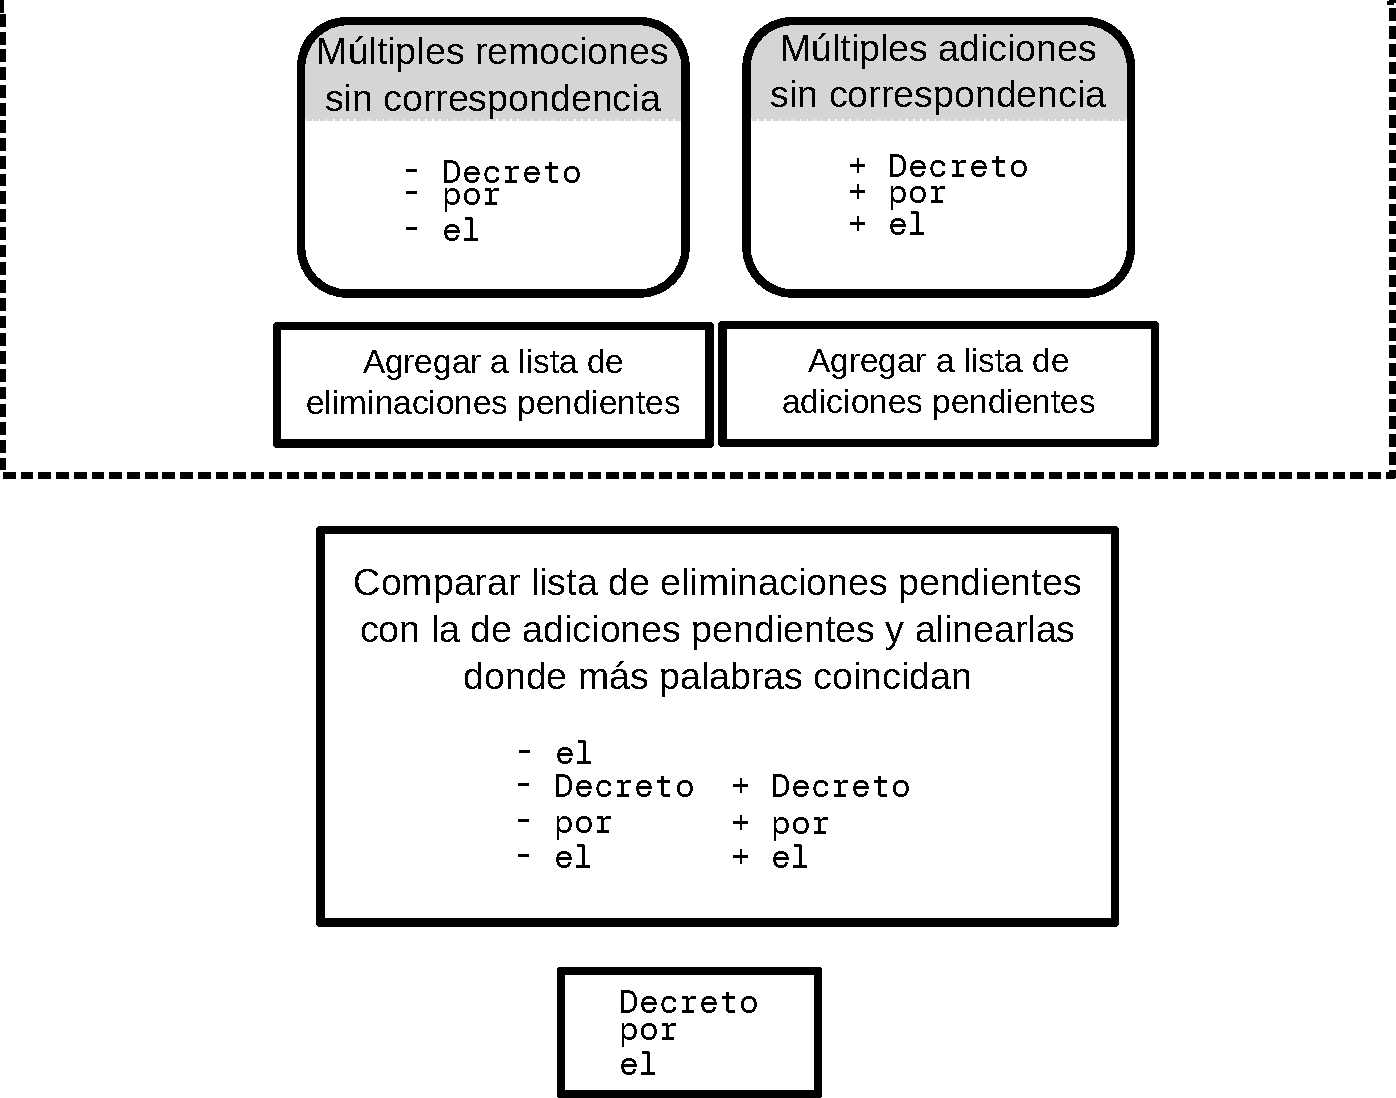
\includegraphics[width = 0.8\textwidth]{\DirFigCtres/combinacion_texto_ocr_2}
    \caption{Detalle de combinación de teto plano con información de OCR (Pt 2).}
    \label{fig:esquema_combinacion_txt_ocr_2}
\end{figure}

Al terminar el proceso se tiene un arreglo de datos donde se conoce la posición
y dimensiones de cada palabra, así como su texto correcto, además se cuenta con
datos adicionales de linea, columna, alineación o grupo que serán empleadas
para dividir las secciones del documento más adelante.

Las ventajas de usar PdfPlumber sobre PyPDF+PyTesseract son que es más rápido y
la identificación del texto es certera, pues proviene directamente del archivo,
sin embargo, no funciona si el PDF es un escaneo o si contiene texto en forma
de imagen.

Por su parte, al generar el método que emplea PyPDF+PyTesseract, se desarrollaron
elementos que fueron reciclados, como la resconstrucción de texto, además de
que puede funcionar en documentos escaneados (confiando completamente en la
predicción de PyTesseract) y documentos con imágenes, además de que es mejor
eliminando texto no visible en el PDF.

\subsection{Obtener estructura del documento}

El objetivo de este paso es generar una estructua de datos en la que cada parte
del documento esté referenciada a su sección y subsecciones correspondientes,
por ejemplo, para la Ley Orgánica deseamos conocer en qué título, capítulo y
artículo se encuentra un texto específico.

Para realizar dicha estructura se optó por generar un árbol, donde cada nodo
corresponde a una sección del documento, además, las hojas y los nodos intermedios
almacenan el texto de cada artículo o sección según sea el caso. En la figura
\ref{fig:fragmento_arbol} se muestra un fragmento del árbol correspondiente a
las primeras secciones de la Ley Orgánica.

\begin{figure}[]
    \centering
    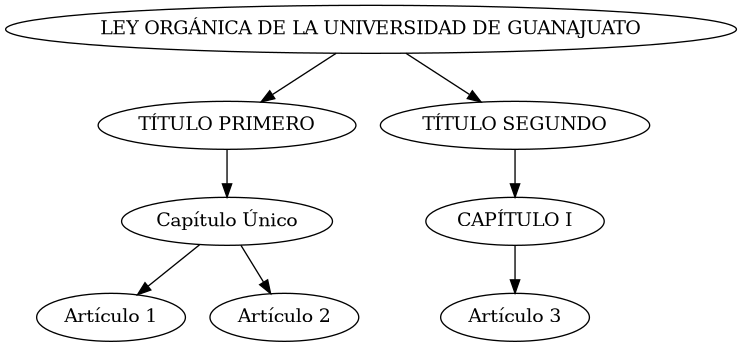
\includegraphics[width = 0.8\textwidth]{\DirFigCtres/fragmento_arbol}
    \caption{Fragmento de árbol de documento 'Ley Orgánica de la Universidad de Guanajuato'.}
    \label{fig:fragmento_arbol}
\end{figure}

Para generar el árbol es necesario analizar el documento en varios pasos. Primero,
se detectan las líneas o fragmentos que corresponden a títulos, estas típicamente
se encuentran centrados en la página o en la columna, a los primeros se les
asigna el tipo 1 y a los segundos el tipo 2, el texto restante tendría tipo 0.
Para que el fragmento sea considerado como título deberá haber un espacio
vertical antes o después dependiendo del tipo.

Para encontrar las secciones o subsecciones se consideran los títulos
centrados en la página (tipo 1), a los cuales se les asigna un nivel. Para asignar
el nivel a un título es necesario conocer de antemano la estructura del
documento, específicamente, se debe crear una expresión regular para
identificar cada nivel. Por ejemplo, para la Ley Orgnánica de la Universidad
de Guanajuato la estructura que se tiene es la siguiente:

\begin{enumerate}
    \item Encabezado general: Son títulos abiertos que no tienen palabras o
          estructura específica y se consideran dentro del primer nivel.
          \begin{itemize}
              \item Sin expresión regular
          \end{itemize}
    \item Título: El documento se divide en títulos. Cada título comienza con
          la palabra \textit{Título}.
          \begin{itemize}
              \item \string^(título\textbar[xiv]+\textbackslash.) .*
          \end{itemize}
    \item Capítulo: Los títulos se dividen an capítulos y cada capítulo comienza
          con la palabra \textit{Capítulo}
          \begin{itemize}
              \item \string^capítulo .*
          \end{itemize}
\end{enumerate}

Además, se debe tener en cuenta que hay divisiones del documento
que no se encuentran centrados, sino que están contenidos en el grueso del
texto, como lo son los Artículos. Para identificar estas separaciones en el
contenido, también se crean expresiones regulares que se verifican contra el
inicio de cada línea mientras se va construyendo el árbol.

\begin{enumerate}
    \item Artículo: Los capítulos tienen uno o más artículos.
          \begin{itemize}
              \item  \string^artículo ([0-9]+\textbar[a-zé]+(ro\textbar do\textbar ro\textbar to\textbar mo\textbar vo\textbar no\textbar único)\\
                    (bis\textbar ter\textbar quáter\textbar quinquies)?\textbackslash.
          \end{itemize}
\end{enumerate}

Una vez identificados los títulos y teniendo la forma para encontrar las
divisiones dentro del contenido, se recorre el documento. Recorrer
el documento es el equivalente a recorrer el árbol por profundidad, por lo
que se va creando el árbol de la misma forma, es decir, cuando se encuentra
un título se crea un nuevo nodo en el nivel correspondiente, siempre teniendo
la referencia de cual será su padre, cuando se llega al nivel más bajo se
guarda el contenido de texto en el nodo correspondiente.
El proceso completo se presenta en la figura
\ref{fig:crear_arbol}.

\begin{figure}[]
    \centering
    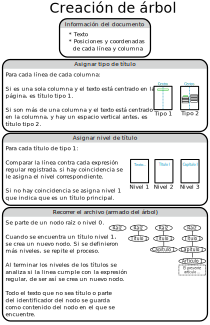
\includegraphics[width = 0.8\textwidth]{\DirFigCtres/crear_arbol}
    \caption{Proceso de creación del árbol de secciones de un documento.}
    \label{fig:crear_arbol}
\end{figure}

\subsection{Obtener \textit{embeddings}}

Para el cálculo de \textit{embeddings} se emplean LLMs especializados,
estos modelos son entrenados en datasets de similitud semántica o QA en
diferentes idiomas. El sistema propuesto permite el uso y evaluación de
varios modelos, los cuales serán: MiniLM (33M de parámetros)
\cite{wang_minilm_2020}, MPNET \cite{hagen_mpnet_2020} (110M de parámetros)
y Qwen 3 \cite{zhang_qwen3_2025} (600M, 4B y 8B de parámetros). Estos modelos
se encuentran disponibles en HuggingFace para su descarga y se pueden
emplear a través de la librería \textit{SentenceTransformers}, la cual está especializada
en obtener embeddings de oraciones.

Los modelos MiniLM y MPNET fueron seleccionados por su tamaño reducido,
ya que incluso pueden correr en CPU de forma eficiente, mientras que los
modelos Qwen fueron seleccionados porque ocupan los primeros puestos en el
MTEB Ladderboard de HuggingFace \footnote{https://huggingface.co/spaces/mteb/leaderboard},
que clasifica modelos de extracción de \textit{embeddings} en diferentes idiomas
y con múltiples métricas.

En el caso de los modelos Qwen 3, existen versiones cuantizadas de éstos,
las cuales emplean el mismo número de parámetros que su versión original,
pero disminuyendo la precisión de los números flotantes de sus parámetros.
Para el caso de Qwen 3, existen versiones de 16-bits, 8-bits, 6-bits, 5-bits y
4-bits.

**Incluir tabla resumen de modelo, parámetros y tamaño de embeddings.**

El proceso para convertir la información del documento a embeddings consiste
en recorrer el árbol en profundidad, y en cada nodo hacer lo siguiente:

\begin{enumerate}
    \item Tomar el contenido textual del nodo y separarlo por párrafos.
          Cada párrafo será un registro independiente.
    \item Utilizar SentenceTransformers para calcular los embeddings de cada
          párrafo y guardarlo como un vector de números.
    \item Obtener la ruta del nodo dentro del árbol. Ej: Ley Orgánica $\rightarrow$
          Título Primero $\rightarrow$ Capítulo segundo $\rightarrow$ Artículo 30.
    \item Guardar la ruta y el nombre del nodo como metadatos (información
          adicional que se podría usar para filtrar la información).
\end{enumerate}

Al final por cada párrafo del documento se tendrá la siguiente información:

\begin{itemize}
    \item Metadatos:
          \begin{itemize}
              \item Ruta en el árbol
              \item Nombre del nodo
          \end{itemize}
    \item Embedding como vector de N valores numéricos.
\end{itemize}

\subsection{Almacenar información}

Los embeddings pueden almacenarse de varias formas en el disco, sin embargo,
las dos formas más convenientes son: en formato CSV o en una base de datos
que soporte vectores.

El formato CSV tiene la ventaja de ser portable y facil de leer, lo único que
hay que hacer es convertir los metadatos a formato JSON, así podrán ser
almacenados como texto, mientras que el vector de embeddings se puede
expandir y crear una columna para cada valor. En la figura \ref{fig:ejemplo_csv}
se muestra un ejemplo de la información almacenada como archivo CSV.

\begin{figure}[]
    \centering
    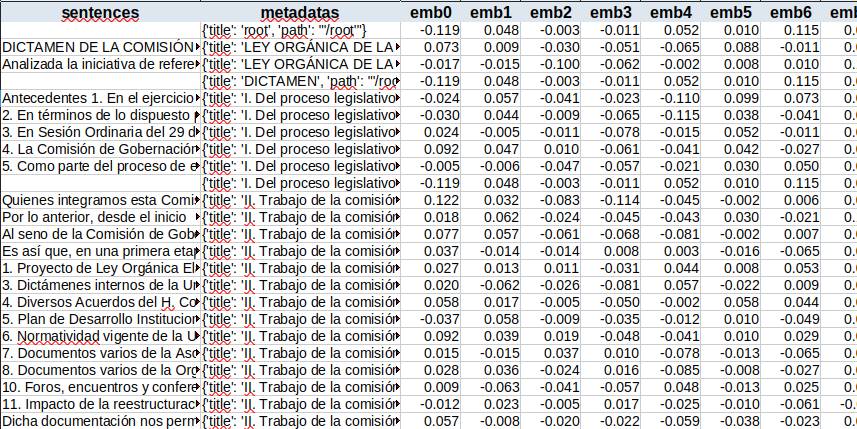
\includegraphics[width = 0.8\textwidth]{\DirFigCtres/ejemplo_csv}
    \caption{Ejemplo de cómo se almacenan metadatos y embeddings en formato csv.}
    \label{fig:ejemplo_csv}
\end{figure}

Sin embargo, este método no es apto para entornos productivos, ya que no tiene
mecanismos nativos para búsqueda en los vectores de datos.

Otra forma de almacenar los embeddings es empleando una base de datos que
soporte vectores. Existen muchas alternativas y cada una ofrece beneficios
particulares, en general todas permiten almacenar los datos de forma
óptima ya que se pueden organizar en tablas, agregar informació adicional y
tienen implementadas funciones de búsqueda por similitud de vectores.
Algunos ejemplos de estas bases de datos vectoriales son: Chroma, Marco,
PostgreSQL, entre otras.

ChromaDB es una base de datos de vectores diseñada para funcionar en
entornos productivos, e incluye mecanismos para calcular los embeddings
empleando \textit{SentenceTransformers} u otro método personalizado, además,
permite el uso de diferentes parámetros de búsqueda por similitud semántica
como son la distancia coseno y el producto interno, los cuales también se
encuentran optimizados. En la figura \ref{fig:ejemplo_chromadb} se muestra
un ejemplo de datos almacenados en ChromaDB.

\begin{figure}[]
    \centering
    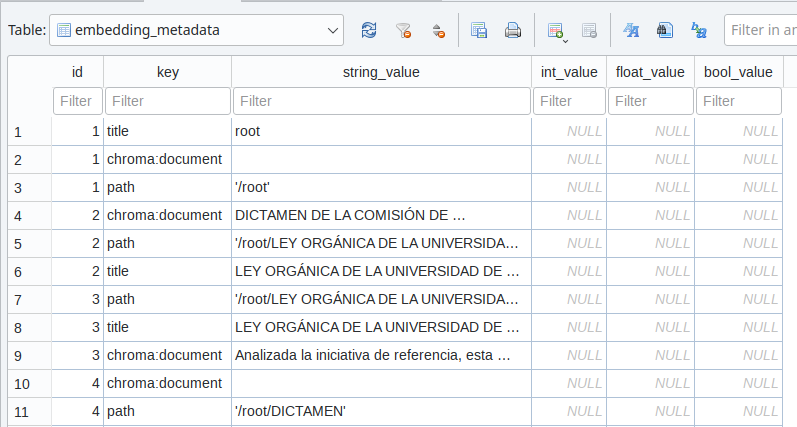
\includegraphics[width = 0.8\textwidth]{\DirFigCtres/ejemplo_chromadb_1}
    \caption{Ejemplo de cómo se almacenan metadatos en Chroma DB. Los vectores
        se almacenan en un lugar no visible para el usuario.}
    \label{fig:ejemplo_chromadb}
\end{figure}

\section{Modelador de lenguaje}

El modelador de lenguaje tiene dos funciones fundamentales: manejar la
interacción con la base de datos de vectores y manejar la interacción con el
LLM principal, en términos de RAG, se encarga de la recuperación y la
generación.

El proceso general que ejecuta el modelador de lenguaje se presenta en el
diagrama de la figura \ref{fig:esquema_modelador} y se explica a continuación.

\begin{figure}[]
    \centering
    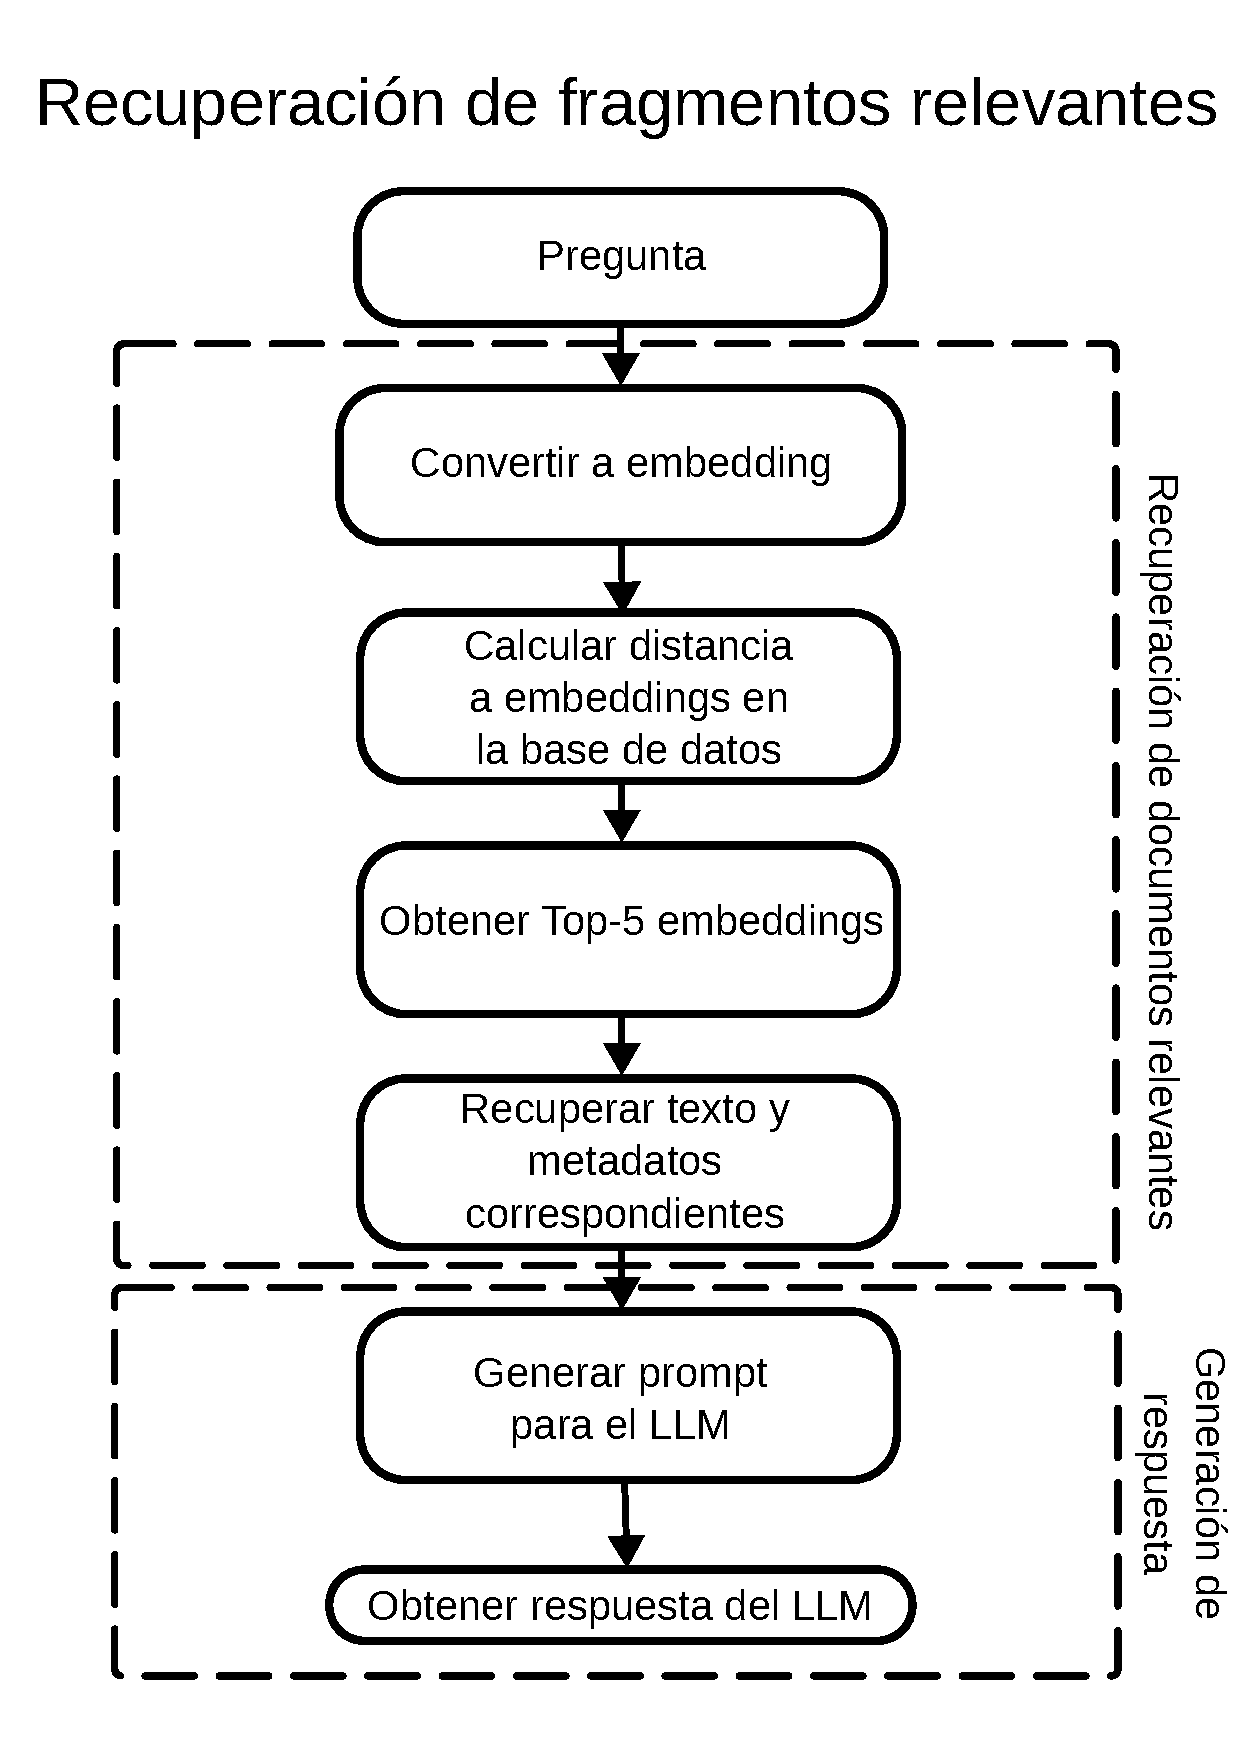
\includegraphics[width = 0.8\textwidth]{\DirFigCtres/esquema_recuperacion}
    \caption{Pasos seguidos por el modelador de lenguaje para procesar una pregunta.}
    \label{fig:esquema_modelador}
\end{figure}

\subsection{Recuperación de documentos relevantes}

Dada una pregunta o \textit{query}, el modelador la convierte a \textit{embedding}
empleando el mismo modelo usado para la base de datos. Este \textit{embedding}
se le proporciona a ChromaDB para hacer la búsqueda semántica, el parámetro
de búsqueda puede ser por producto interno o por similitud coseno, dependiendo
del modelo de \textit{embeddings}. Para hacer una búsqueda eficiente,
ChromaDB emplea un índice llamado HNSW (Hierarchical Navigable Small World),
esto le permite buscar de forma eficiente la similitud con todos los registros.

Con ChromaDB se obtiene el top \textit{k} de \textit{embeddings} similares,
por defecto \textit{k} se establece en 5. De estos \textit{k} \textit{embeddings}
se obtiene su texto original, su posición dentro del árbol del documento, el
documento al que pertenece y los demás metadatos.

\subsection{Generación de respuesta}

Para la generación de la respuesta, se emplean modelos multidominio de código
abierto, la intención es comparar modelos de diferentes tamaños para
encontrar el óptimo. Se evaluan los modelos Qwen 3 \cite{zhang_qwen3_2025}
(600M, 4B y 8B de parámetros) en sus versiones completas y cuantizadas,
Llama 3.1 (1B, 3B y 8B de parámetros) en sus versiones completas y cuantizadas
y Gemma 3 (1B, 4B, 12B y 27B de parámetros) en sus versiones completas y
cuantizadas.

**Agregar tabla comparativa de modelos**

A todos los modelos se les configura una instrucción de sistema indicando
que su propósito es proporcionar ayuda sobre la normativa y se le indican
algunos lineamientos de comportamiento.

**Agregar prompt del sistema con instrucciones**

Una vez se tiene una pregunta y sus los fragmentos relevantes, se extrae
tanto el texto como sus metadatos, los cuales incluyen: el documento, artículo
o sección, y, en algunos casos, el subtítulo o nombre de sección.
Con el fin de transmitir esta información al LLM, se crea una plantilla de
\textit{prompt} que contiene la pregunta, los documentos relevantes y la
instrucción de responder la pregunta con el contexto proporcionado.

**Agregar plantilla del prompt.**

Una vez generado el \textit{prompt} se le manda al LLM, junto con el historial
anterior del chat en caso de existir, y se espera por la respuesta.

\section{API de comunicación}

**Reemplazar esta sección con la documentación formal de la API**

La tarea de la API es conectar la aplicación web con el modelador de lenguaje.
La API funciona con peticiones http de tipo POST y conste en un solo endpoint
el cual recibe el nombre del modelo y la lista de mensajes entre el
usuario y el modelo, cada mensaje se identifica con un rol para distinguir
los mensajes del usuario de las respuestas del modelo. Las peticiones se
manejan en formato JSON como se muestra en la figura \ref{fig:parametros_api}.

\begin{figure}[]
    \centering
    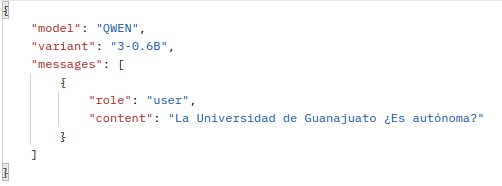
\includegraphics[width = 0.8\textwidth]{\DirFigCtres/parametros_api}
    \caption{Ejemplo de petición a API.}
    \label{fig:parametros_api}
\end{figure}

La respuesta de la API también es en formato JSON y contiene el texto de la
respuesta, así como los documentos que fueron tomados como contexto para
emitirla, como se muestra en la figura \ref{fig:respuesta_api}. En estos
documentos, se incluyen los metadatos para poder desplegarlos en la aplicación
web.

\begin{figure}[]
    \centering
    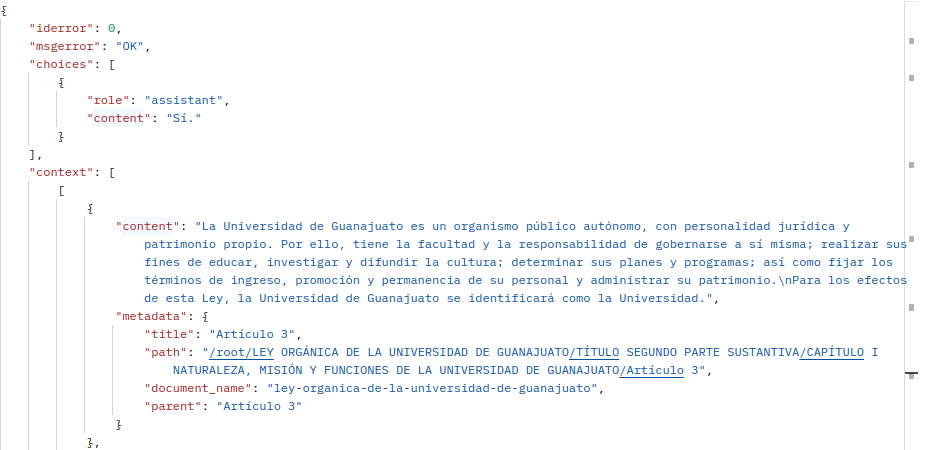
\includegraphics[width = 0.8\textwidth]{\DirFigCtres/respuesta_api}
    \caption{Ejemplo de respuesta de API.}
    \label{fig:respuesta_api}
\end{figure}

Por último, para garantizar la seguridad en el acceso de la API, se implementa
un sistema de autenticación por API-Key, la cual es un token que debe
enviarse en el encabezado 'api-key' de la petición.

\section{Aplicación web}

La aplicación web es la única fuente de interacción de los usuarios con el
sistema, es por ello que debe contener todas las funcionalidades necesarias
que en este caso son: Ingresar una pregunta, recibir una respuesta y
consultar los documentos que dan fundamento a dicha respuesta.

Es bajo esta premisa que se desarrolla una aplicación web con una interfaz
que contiene una caja de texto para hacer la pregunta y despliega la
lista de mensajes y respuestas como un chat convencional. Adicionalmente
se destina un espacio para colocar los documentos relacionados con la
pregunta, como se muestra en la figura \ref{fig:pregunta_web}.

\begin{figure}[]
    \centering
    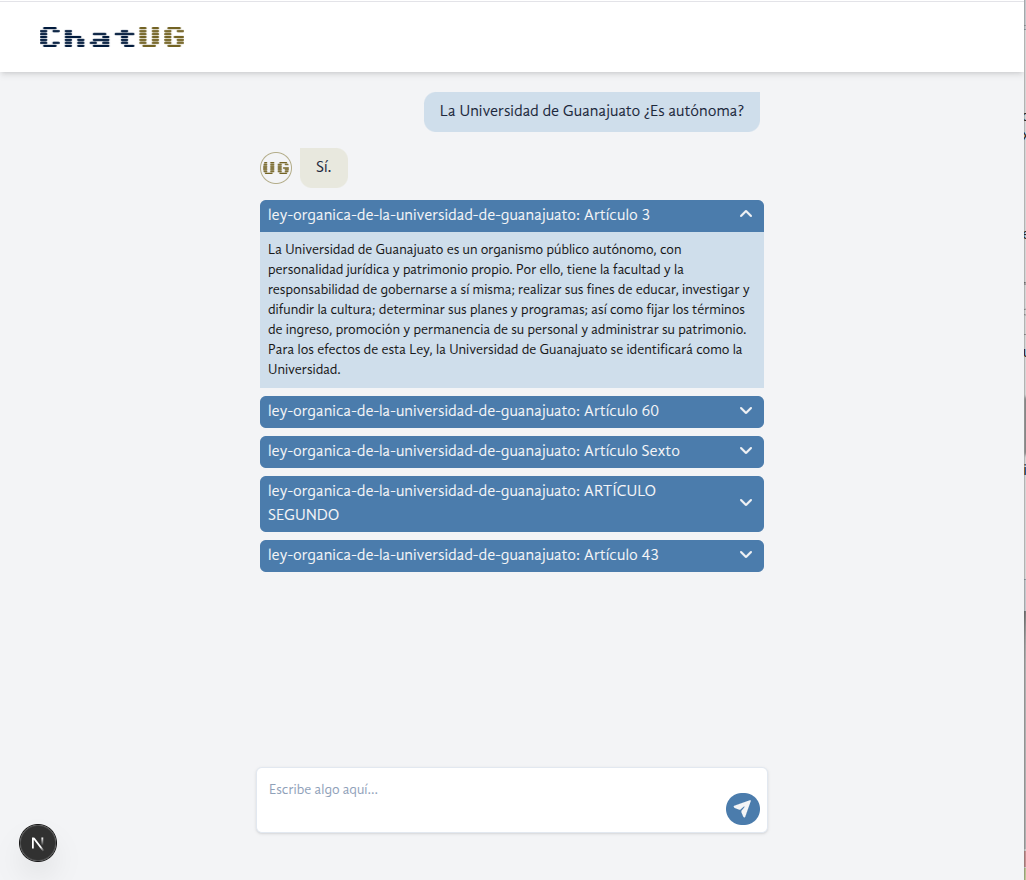
\includegraphics[width = 0.8\textwidth]{\DirFigCtres/pregunta_web}
    \caption{Ejemplo de pregunta a través de aplicación web. **Reemplazar
        esta imagen con el wireframe o prototipo de la aplicación**}
    \label{fig:pregunta_web}
\end{figure}
